\backgroundsetup{
  scale=1,
  opacity=0.6,
  angle=0,
  % contents={\includegraphics[width=\paperwidth]{images/bild.jpg}}
}

\begin{titlepage}
  \pagecolor{black}
  \color{white}

  \centering

  {\scshape\LARGE Maturaarbeit\par}
  \vspace{1cm}
  {\huge\bfseries Maschinelles Lernen mit TensorFlow\par}
  \vspace{0.2cm}
  {\large Entwicklung eines Convolutional Denoising Autoencoders\par}
  \vfill
  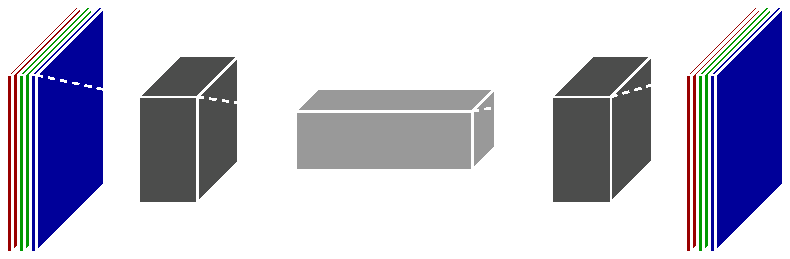
\includegraphics[width=0.9\textwidth]{titel.pdf} \par
  \vspace{1cm}
  {\Large\itshape Luis Wirth\par}
  \vfill
  \vspace{2cm}
  {\scshape\Large Gymnasium Oberwil\par}
  {\large Klasse \textit{4a}\par}
  \vspace{2cm}
  Betreut von\par
  Dr. Jonas \textsc{Gloor}

  \vfill
  {\large Abgegeben im September 2019\par}
\end{titlepage}

\pagecolor{pagecolor}
\color{textcolor}

\addcontentsline{toc}{chapter}{Inhaltsverzeichnis}
\tableofcontents

\pagebreak


\chapter*{Vorwort}
\addcontentsline{toc}{chapter}{Vorwort}
\section*{Persönliche Themenwahl}
Maschinelles Lernen (machine learning, kurz: ML) stösst seit einigen Jahren auf grosses
Interesse sowohl in der Wissenschaft, als auch in der Wirtschaft. Dies
motivierte mich, Näheres im Selbststudium darüber in Erfahrung bringen zu wollen.
Bereits im Jahr 2017 begann ich, eine erste eigene Applikationen zu programmieren, welche
einen Genetischen Algorithmus zur Anwendung brachte (Evolutionäre Entwicklung
von lernfähigen Agenten). \\
Diese erste Erfahrung öffnete mir die Tür für ein Praktikum am Departement für
Computational Sciences der Universität Basel.
Dort durfte ich ein Künstliches Neuronales Netz
in C++ programmieren, welches ich dann auf eine konkrete physikalische
Problemstellung anwenden konnte (Vorhersage zu den Energiezuständen von
Wassermolekülen in verschiedenen atomaren Konfigurationen). \\
Dieses erste Praktikum hatte mich dazu motiviert, mich tiefgehender mit der Thematik zu befassen
und die grundlegende Funktionsweise von ML durchdringen zu wollen.
\para{}
Daraufhin entstand die Idee, die vorliegende Arbeit zu verfassen.
Auf diese Weise wollte ich mir ein ausgeprägteres mathematisches
Verständnis für Maschinelles Lernen aneignen und auch fortgeschrittene
Modelle betrachten. Zudem hatte ich auch schon von den verbeiteten
Deep-Learning-Frameworks TensorFlow und Keras gehört, welche ich unbedingt
erlernen wollte. Daher entschied ich mich, einen Convolutional-Autoencoder in
TensorFlow zu programmieren und vorher die nötige Theorie zu erklären.
Zuerst verfolgte ich das Ziel, diesen Autoencoder als ein generatives Modell zu entwickeln,
um Bilder von künstlich generierten menschlichen Gesichter zu erzeugen.
\para{}
Während meiner Sommerferien konnte ich ein 6-wöchiges Praktikum im
Forschungszentrum von Adobe in San Francisco leisten, wo ich ebenfalls ein
ML-Modell programmiert habe (Nutzung von Gesichtserkennung für Marketing-Zwecke).
Durch meine praktikumsbezogenen Recherchen gelangte ich jedoch schnell zu der
Erkenntnis, dass mein ursprüngliches ambitiöses Vorhaben bezüglich der generativen Nutzung eines
Autoencoder den vorgegebenen Rahmen einer Maturaarbeit deutlich sprengen würde.
Ich hätte nämlich nicht nur einen Autoencoder programmieren müssen, sondern
sogar einen Variational Autoencoder, welcher mathematisch noch deutlich
anspruchsvoller gewesen wäre.
\para{}
Aus diesem Grund beschloss ich, meine Leitfrage in Abstimmung mit meiner
Betreuungsperson anzupassen. Diese beschränkt sich nunmehr auf die Entwicklung
eines Convolutional \textit{Denoising} Autoencoder in TensorFlow und Keras sowie
vorgängig die zugrundeliegende Theorie zu erklären.

\section*{Danksagung}
Mein herzlicher Dank gilt dem Department für Computational Sciences der
Universität Basel, namentlich Herrn Professor Stefan Goedecker, weil er und sein Team
mir die ersten wissenschaftliche Einblicke in das Thema Machine Learning
eröffnet haben. \\
Danken möchte ich ebenso der Firma Adobe, welche mir ermöglicht hat, im Rahmen
eines 6-wöchigen Praktikums die kommerzielle Anwendung von Machine Learning
vertieft kennenzulernen. \\
Ebenso danke ich meinen Eltern, Frau Dr. Doris Fellenstein und Herrn Dr. Victor
Wirth für ihre Begleitung und Unterstützung während des Erstellungsprozesses
meiner Maturaarbeit. \\
Last but not least gilt mein besonderer Dank meiner Betreuungsperson Herrn Dr. Jonas
Gloor für seine wertvollen fachlichen Inputs.

\chapter*{Einleitung}
\addcontentsline{toc}{chapter}{Einleitung}
Maschinelles Lernen erfreut sich aktuell grosser Beliebtheit und wird
sehr erfolgreich in naturwissenschaftlichen, medizinischen oder auch
wirtschaftlichen Themenbezügen angewendet. Es bietet ein enormes
Innovationspotential und wird laufend weiterentwickelt.
Obwohl das Schlagwort ``Künstliche Intelligenz'' in aller Munde ist, wissen die
Wenigsten, wie sie tatsächlich funktioniert.
\para{}
Das Ziel dieser Arbeit ist daher, dem Leser ein umfassendes Grundverständnis
über Maschinelles Lernen zu vermitteln, sowie auf dieser Basis ein konkretes
Anwendungsbeispiel zu entwickeln. Zu diesem Zweck werden zunächst die
theoretischen Grundlagen zum modellbasierten Lernen dargelegt. Darauf aufbauend
ist es möglich, ein konkretes Modell, namentlich Künstliche Neuronale Netze
(KNN), in
ihrer Funktionsweise zu erläutern. In logischer Konsequenz wird anschliessend
die spezifische Architektur eines KNNs präsentiert. Namentlich handelt sich um
ein Convolutional Neural Networks (CNN), welches sich besonders gut für
Bildverarbeitungszwecke eignet und daher eine grosse Verbreitung in der Praxis aufweist.
Mit der anschliessenden Erläuterung der mathematischen Beschreibung eines Autoencoders sind
die theoretischen Grundlagen für ein konkretes Anwendungsbeispiel geschaffen.
\para{}
Nachdem ein mathematisch fundiertes Verständnis für Maschinelles Lernen
vermittelt wurde, sollen im Weiteren zwei Open-Source Implementationen vorgestellt
werden. Dabei handelt es sich um TensorFlow, ein ursprünglich von Google
entwickeltes Framework für Deep-Learning, und um Keras, eine übergeordnete
Schnittstelle für eine vereinfachte TensorFlow-Verwendung. Neben ihrer grossen
Verbreitung besitzen sie den Vorteil eines verkürzten Einstiegs in die
ML-Programmierung.
\para{}
Für das konkrete Modell werden wir einen sogenannten
Convolutional-Denoising-Autoencoder entwickeln. Mit dessen Hilfe kann das
Bildrauschen von Bildern entfernt werden. Eine beispielhafte
Anwendungsmöglichkeit bildet das korrekte Einlesen von standardisierten (verrauschten) Formularen.
\para{}
Die Leitfrage lässt sich demnach folgendermassen formulieren:
\begin{center}
 \textbf{Wie funktioniert Maschinelles Lernen, aufgezeigt anhand eines konkreten
   Modells, unter Verwendung von TensorFlow und Keras?}
\end{center}
\para{}
Dabei lassen sich folgende Teilschritte unterscheiden:
\begin{enumerate}
  \item{Erarbeiten der allgemeine Theorie zum Maschinellen Lernen}
  \item{Künstliche Neuronale Netze als Modelle für ML}
  \item{Convolutional Neural Networks und Autoencoder als konkrete KNN-Architekturen}
  \item{Grundsätzliche Funktionsweise der ML-Frameworks TensorFlow und Keras}
  \item{Programmierung eines konkreten ML-Modells mit TensorFlow und Keras}
\end{enumerate}



\chapter*{Konvention und Notation}
\addcontentsline{toc}{chapter}{Konvention und Notation}

\subsection*{Beschriftung}

\begin{center}\textbf{Zahlen und Tensoren}\end{center}
\begin{tabular}{cl}
  $a$ & ein Skalar (Zahl) \\
  $\vec{a}$ & ein Vektor \\
  $\vec{a} \in \set{R}^{n}$ & ein Vektor mit $n$ Komponenten \\
  $\mat{A}$ & eine Matrix \\
  $\mat{A} \in \set{R}^{m \times n}$ & eine Matrix mit $m$ Zeilen und $n$ Spalten \\
  $\ten{A}$ & ein[x={(0.866cm,0.5cm)}, y={(-0.866cm,0.5cm)}, z={(0cm,1cm)}, scale=0.7] Tensor \\

\end{tabular}

\begin{center}\textbf{Mengen}\end{center}
\begin{tabular}{cl}
  $(a,b)$ & ein geordnetes Paar (2-Tupel) der Elemente $a$ und $b$ \\
  $\set{A}$ & eine Menge \\
  $\set{R}$ & die Menge aller reellen Zahlen \\
  $\set{Z}$ & die Menge aller ganzen Zahlen \\
  $\set{N}$ & die Menge aller natürlichen Zahlen \\
  $\{a,b\}$ & die Menge, welche aus den Elementen $a$ und $b$ besteht \\
  $\{1,\ldots,n\}$ & die Menge aller ganzen Zahlen von 1 bis $n$ \\
  $a \in \set{A}$ & $a$ ist ein Element der Menge $\set{A}$ \\

\end{tabular}

\begin{center}\textbf{Indexierung}\end{center}
\begin{tabular}{cl}
  $\vecelem{a}_i$ & die $i$-te Vektorkomponente mit Startindex 1 \\
  ${(\mat{A})}_{i,j}$ & das Matrixelement in der $i$-ten Zeile und der $j$-ten Spalte \\
  $\matelem{A}_{i,j}$ & das Matrixelement in der $i$-ten Zeile und der $j$-ten Spalte \\
  $\mat{A}_{i,:}$ & die Zeile $i$ der Matrix $\mat{A}$ \\
  $\mat{A}_{:,i}$ & die Spalte $i$ der Matrix $\mat{A}$\ \\
  $\ten{A}_{i,:,:}$ & der $i$-te Querschnitt entlang der Höhe des Tensors $\ten{A}$ \\
  $\ten{A}_{:,i,:}$ & der $i$-te Querschnitt entlang der Breite des Tensors $\ten{A}$ \\
  $\ten{A}_{:,:,i}$ & der $i$-te Querschnitt entlang der Tiefe des Tensors $\ten{A}$ \\
\end{tabular}

\begin{center}\textbf{Lineare Algebra Operationen}\end{center}
\begin{tabular}{cl}
  $\Sigma(\mat{A})$ & die Summe aller Elemente von Matrix $\mat{A}$ \\
  $\vec{v} \cdot \vec{w}$ & das Skalarprodukt von $\vec{v}$ mit $\vec{w}$ \\
  $\trans{\mat{A}}$ & das Transponierte einer Matrix $\mat{A}$ \\
  $\mat{A} \odot \mat{B}$ & das elementeweise (Hadamard) Produkt \\
  $\mat{A} * \mat{B}$ & die diskrete Faltung von $\mat{A}$ ueber $\mat{B}$

\end{tabular}

\begin{center}\textbf{Infinitesimalrechnung}\end{center}
\begin{tabular}{cl}
  $f'(x)$ & die Ableitung der Funktion $f$ bezüglich seinem Argument $x$ \\
  $\ds\deriv{y}{x}$ & die Ableitung von $y$ bezüglich $x$ \\[2ex]
  $\ds\partderiv{y}{x}$ & die partielle Ableitung von $y$ bezüglich $x$ \\[2ex]
  $\vecf{\nabla} y$ & der Gradient von $y$\\
  $\vecf{\nabla}_{\vec{x}}y$ & der Gradient von $y$ bezüglich $\vec{x}$ (Vektor) \\
  $\ds\int f(x)\,\text{d}x$ & das unbestimmte Integral der Funktion $f$ bezüglich $x$ \\
  $\ds\int_a^b f(x)\,\text{d}x$ & das bestimmte Integral der Funktion $f$ bezüglich $x$ von $a$ bis $b$ \\
  $\ds\lim_{x \to a} f(x)$ & der Limes/Grenzwert von $f$, wenn $x$ gegen $a$ strebt \\

\end{tabular}

\begin{center}\textbf{Funktionen}\end{center}
\begin{tabular}{cl}
  $f: \set{A} \to \set{B}$ & eine Funktion $f$ mit Definitionsmenge $\set{A}$ und Zielmenge $\set{B}$ \\
  $f(x)$ & eine Funktion $f$ mit Argument $x$ (Skalar) \\
  $f(\vec{v})$ & eine Funktion $f$ mit Argument $\vec{v}$ (Vektor) \\
  $\vecf{f}[\vec{v}]$ & die vektorisierte Funktion $\vecf{f}$ mit Argument $\vec{v}$ (Vektor) \\
  $\mathcal{A}$ & ein Funktionenraum \\
  $f * g$ & die Faltung von $f$ über $g$ \\
  $f \circ g$ & die Komposition von den Funktionen $f$ und $g$ \\

\end{tabular}

\begin{center}\textbf{Statistik}\end{center}
\begin{tabular}{cl}
  $\mathcal{N}$ & die Gauss'sche Normalverteilung \\
  $\phi$ & die Gauss'sche Dichtefunktion \\
  $\mu$ & der Erwartungswert/Mittelwert \\
  $\sigma$ & die Standardabweichung \\
  $\sigma^2$ & die Varianz
\end{tabular}

\begin{center}\textbf{Sonstiges}\end{center}
\begin{tabular}{cl}
  $\ds\sum_{i=a}^b x$ & die Summe mit von $a$ bis $b$ ueber $x$ mit Laufvariable $i$ \\
\end{tabular}

Erwähnung von Notation $\set{R}$ für Skalare und $\set{R}^n$ für Vektoren/Vektorräume...

%%% Local Variables:
%%% mode: latex
%%% TeX-master: "../main"
%%% End:

% LocalWords:  ML machine Themenwahl
